\chapter{From formal boosted tree explanations to
interpretable rule sets} \label{chap:cp23}

This chapter is based on:
\begin{itemize}
	\item Jinqiang Yu, Alexey Ignatiev, and Peter J. Stuckey. From formal boosted tree explanations to
interpretable rule sets. \emph{In 29th International Conference on Principles and Practice of
	Constraint Programming,} vol. 280, pp.38:1-38:21, 2023.
\end{itemize}

Explaining decision sets is notably straightforward: the rule that ``fires'' a given instance
serves as the explanation for that instance.
%
This led to increased interest in decision sets that are both easy to understand
to accurate.
%
The method presented in \autoref{chap:jair21} produces decision sets of minimum size that achieve
perfect accuracy on the training data and demonstrates that decision sets that fully align with the
training data exhibit superior accuracy compared to others.
%
A more scalable method~\cite{ilsms-aaai21} to generate perfectly accurate decision sets was the
introduced.
%
However, neither of these methods can offer any decision information if a dataset is not entirely solved.
%
Inspired by these studies and their limitations, this chapter focuses on establish a connection between 
formal post-hoc explainability and decision sets.
%
Specifically, this chapter aims to develop an innovative anytime method to generate decision sets that are 
both accurate and interpretable. 
%
This is achieved by distilling a gradient boosted tree model into a decision set on demand with 
the use of abductive explanations~(AXp's).
%
In addition, the chapter introduces several post-hoc model reduction techniques aimed at
improving the interpretability of the result decision sets with the use of MaxSAT and 
integer linear programming~(ILP).
%
Empirical results conducted on various datasets show that our method 
generates decision sets outperforming those produced by state-of-the-art approaches in terms of
accuracy, while remaining comparable regarding explanation size.


%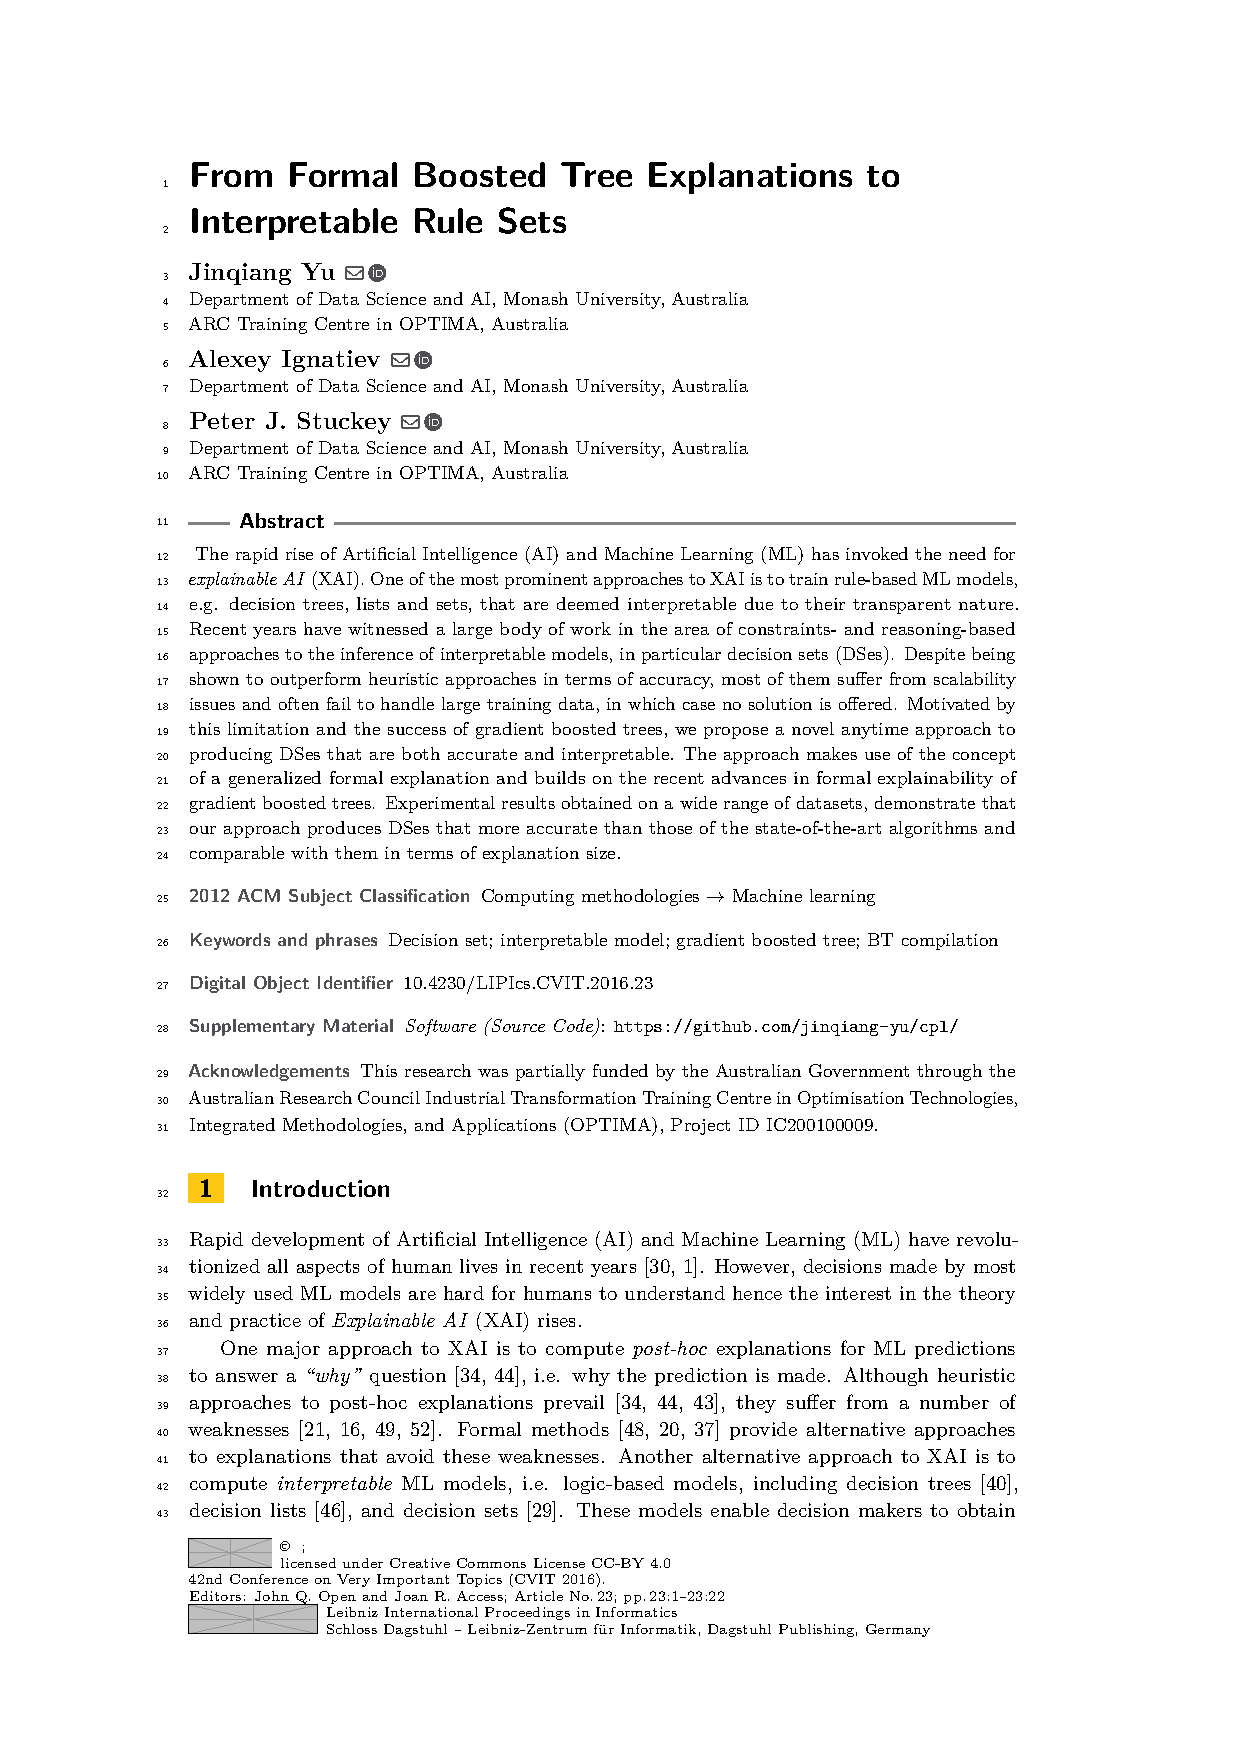
\includepdf[pages=-, offset=75 -75]{papers/cp23.pdf}
